\documentclass[../catalog.tex]{subfiles}

\begin{document}

\subsubsection{Problem}

Recall from chapter \ref{3df-data-model} our opinions on data modeling
needs of tomorrows information systems. In this world of normalized,
attribute-oriented data, relational joins cannot be treated as scary,
exceptional operations, but rather as commonplace, everyday
tools. Even the most basic aggregation of data, obtaining a consistent
view of domain entities over time, requires joining potentially many
attributes.

How to maintain robust, high-arity joins for many concurrent users
with low-latency and high-throughput is perhaps the defining problem
of the 3DF architecture.

As discussed in chapter \ref{known-techniques}, two approaches for
implementing joins of arbitrary arity avail themselves to us. This
section will focus on the traditional one, where n-way joins are
implemented as consecutive two-way joins (\emph{join stages}).

Join operators must maintain state to buffer inputs on either side,
until matching inputs from the other side arrive (and vice versa) or
the epoch closes. Systems like Kafka Streams enforce sliding,
fixed-size window semantics (\cite{kafkadocs}) to bound the state
maintained by a join operator. Differential Dataflow maintains such
state in arrangements (c.f. chapter \ref{background-differential})
that are compacted as the computation makes progress (i.e. epochs are
completed). Differential's \texttt{join} operator will therefore
arrange both of its input collections, should they not already be
available in arranged form.

For higher-arity joins this becomes problematic, because the output of
the first two-way join will be fed as an input into the second two-way
join, and so on. At each stage along the spine (except for the very
last), intermediate join results will therefore be maintained in
arranged form.

Depending on the selectivity of the various join stages, this can lead
to significant space overheads. Worse, in our continous query
processing setting, erroneously estimating intermediate cardinalities
(a very common problem, as we saw in chapter \ref{known-techniques})
will therefore cause disastrous complexity in both time \emph{and}
space.

\begin{figure}[h!]
  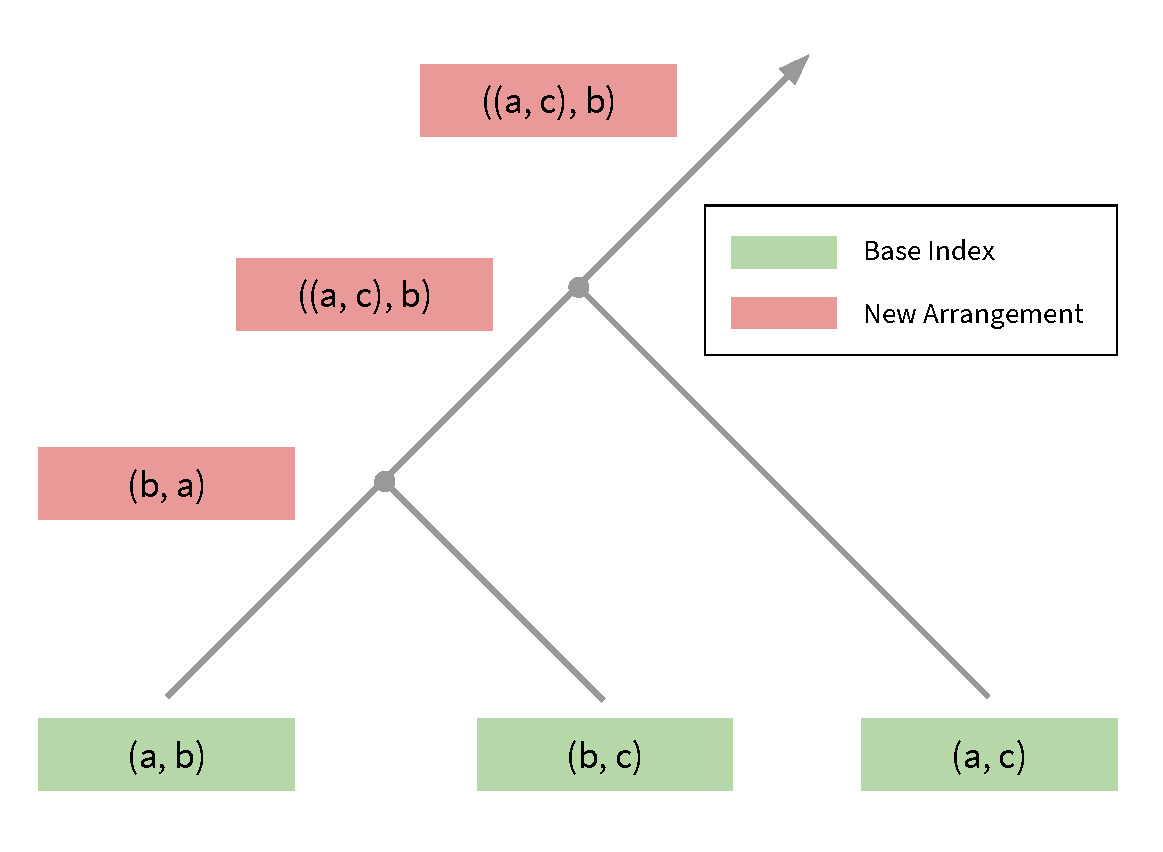
\includegraphics[width=1.0\linewidth]{diagrams/join-at-a-time}
  \caption{Join At A Time}
  \label{fig:join-at-a-time-plan}
\end{figure}

\subsubsection{Example}

Intermediate join state becomes especially apparent in star-joins
along highly correlated columns, e.g. one-to-one relations with very
similar cardinalities and low selectivity. Unfortunately this is a
very common use case in our attribute-oriented data model. Consider
the following query.

\begin{verbatim}
[:find ?comment ?creationDate ?person ?ip ?browser ...
 :where
 [?comment :comment/creation-date ?creationDate]
 [?comment :comment/creator ?person]
 [?comment :comment/ip ?ip]
 [?comment :comment/browser ?browser]
 [?comment :comment/content ?content]
 [?comment :comment/place ?place]]
\end{verbatim}

This query implies a six-way join on the comment ids, aggregating six
different comment attributes back into an aggregate view. Within the
LDBC dataset, every comment carries all six of these attributes,
s.t. all relations are of the same size, and map one-to-one onto each
other. Because of this, implementing this query as five consecutive
two-way joins would lead to roughly a threefold increase in the number
of tuples maintained by this dataflow, \emph{independent of the chosen
  join order}.

We encounter an even more pronounced version of this problem, when
looking at sub-graph queries, such as the triangle search:

\begin{verbatim}
[:find ?a ?b ?c
 :where
 [?a :person/knows ?b]
 [?b :person/knows ?c]
 [?a :person/knows ?c]]
\end{verbatim}

Here the attributes do not have a one-to-one correspondence anymore (a
few celebrities might have in-degrees in the millions, whereas most
people are in mutual friendship with a few hundreds) and join order
becomes crucially important.

\subsubsection{Remedy}

Adapting techniques from the field of incremental view maintenance
(\cite{gupta1993maintaining}, \cite{blakeley1986efficiently}), we can
break up our queries along their potential sources of change. In our
example, any of the comment attributes may change arbitrarily, which
means we will end up with six separate queries.

\begin{figure}[h!]
  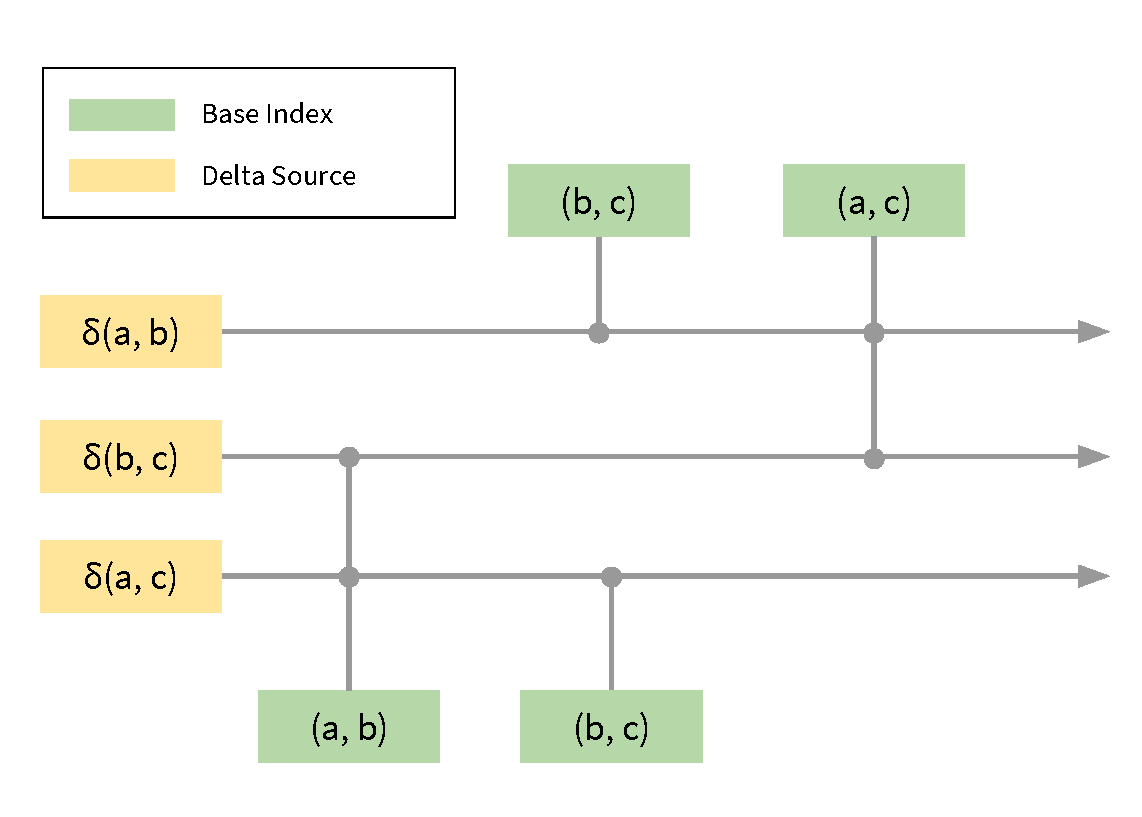
\includegraphics[width=1.0\linewidth]{diagrams/delta-queries}
  \caption{Delta Queries}
  \label{fig:delta-query-plan}
\end{figure}

What is different about the resulting plans, is that, given an indexed
representation of all attributes, they can be implemented in an
otherwise stateless manner. They do not need to maintain intermediate
arrangements as was the case for the traditional join operator.

Assuming for a second that dataflow elements are essentially free
(they are not), this allows us to decouple the memory use of our join
processing from the number of active queries and the complexity of the
joins, and instead bound it in the number and size of attributes
maintained.

There is a trade-off of course, as transforming plans into delta
queries leads to an increase in the number of dataflow elements. We
will see in our discussion of worst-case optimal streaming joins, that
this increase can even be quadratic in the number of relations
involved in the join.

Within any given delta flow, an attribute may only appear at a
position where either of its sides is already bound by the tuples
flowing through it, in order to avoid having to produce the entire
relation for each incoming tuple. We therefore would want to keep
attributes indexed in both directions (from entity id to value and the
other way around), to increase the number of possible plans available
to us.

Another subtle issue, identified in \cite{dogsdogsdogs}, arises when
implementing delta queries within the dataflow model. Simultaneous
updates to multiple of the participating attributes can lead to
redundant derivations of the same result tuple. We must be careful to
impose a logical order on the execution. This implementation detail is
described later in \autoref{impl-altneu}.

\subsubsection{Evaluation}

In order to evaluate the effect of implementing n-way joins with delta
queries, we need to measure the number of tuples maintained across all
active arrangements over the runtime of the system. Differential
provides event streams containing information about the logical size
of trace batches (the data structure backing
arrangements). Differential also provides logging information about
merge events, in which batches that have become indistinguishable
(because the computation frontier has progressed and no operators are
interested in older epochs anymore) are merged together and
compacted. The latter potentially reduces the number of tuples stored
in the system. From those events, the number of tuples across all
arrangements is easily inferred. Implementation details of the logging
instrumentation is covered in chapter \ref{logging}.

We then used the LDBC (\cite{erling2015ldbc}) data generators to
generate a dataset simulating the social network activity of 1000
persons. On this we ran subsets of the above conjunctive query,
increasing the number of clauses participating in the join.

The dataset contains roughly $600,000$ comments.

[@TODO explain constant overhead or fix it...]

\begin{figure}[h!]
  \begin{subfigure}{.5\textwidth}
    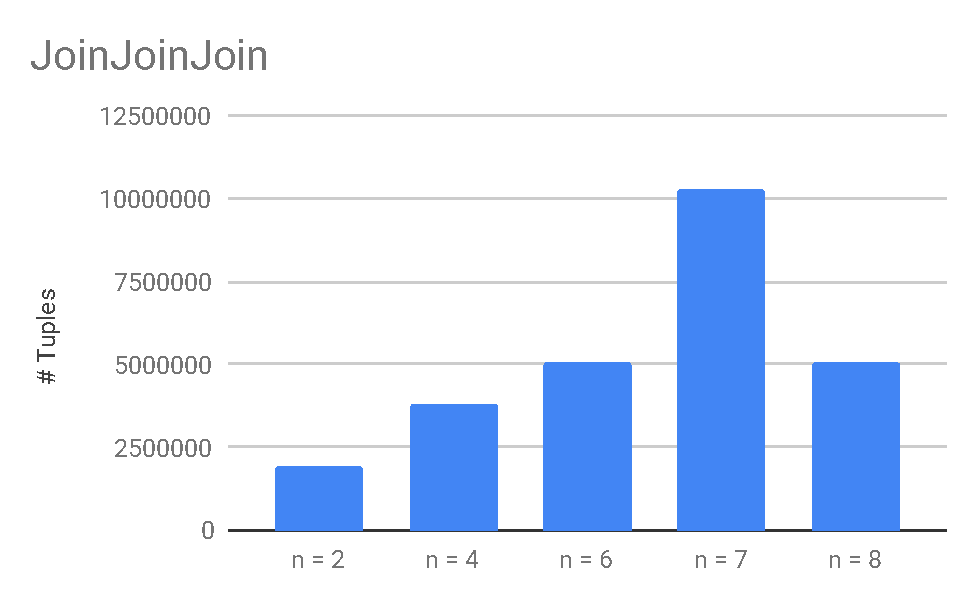
\includegraphics[width=1.0\linewidth]{results/join-state/joinjoinjoin}
    \caption{Consecutive Two-Way Joins}
  \end{subfigure}
  \begin{subfigure}{.5\textwidth}
    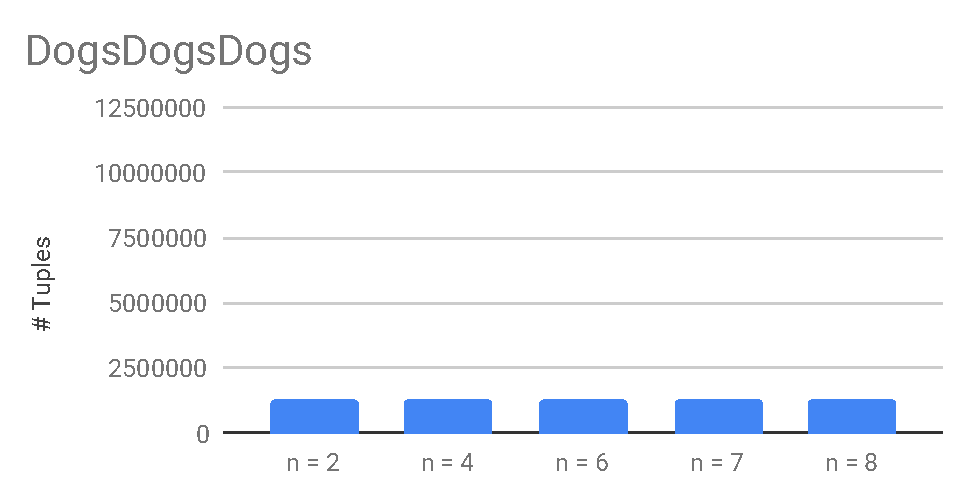
\includegraphics[width=1.0\linewidth]{results/join-state/dogsdogsdogs}
    \caption{Delta Queries}
  \end{subfigure}

  \caption{Total Number of Tuples in Arrangements}
  \label{fig:tuple-counts}
\end{figure}

Figure \ref{fig:tuple-counts} shows the total number of arranged
tuples after each join produced initial results. As expected, we see
that the number of arranged intermediate tuples grows with as more
attributes participate in a consecutive two-way join, whereas it
remains constant when using delta queries.

[@TODO show dataflows and dataflow size]

\subsubsection{Conclusions}

Delta queries allow us to trade dataflow size and a bit of
implementation complexity (due to the lexicograpic timestamps) in
return for predictable memory use. Considering only selections,
projections, and n-way joins, the overall system uses memory
proportional to the number and size of the base relations (i.e. the
individual attributes). No additional operator state is required,
independent of the number of queries and the arity of the joins within
them.

Additionally, delta queries decouple space from time complexity. Using
traditional tree joins, a sub-optimal join plan would incur both a
heavy computational cost as well as space overheads, due to the sheer
number of intermediate tuples materialized and maintained in
arrangements. Delta queries would still have to spend time processing
large numbers of tuples, but without the need to index them.

While we must take measures to keep the overall size of the dataflow
manageable (as will be the topic of later chapters), we conclude that
delta queries are a powerful approach in many common scenarios.

\end{document}
